\documentclass[12pt,a4paper]{article}
\usepackage[utf8]{inputenc}
\usepackage[french]{babel}
\usepackage[T1]{fontenc}
\usepackage{amsmath}
\usepackage{amsfonts}
\usepackage{amssymb}
\usepackage{graphicx}
\usepackage[left=2cm,right=2cm,top=2cm,bottom=2cm]{geometry}
\usepackage[thinspace,thinqspace,amssymb]{SIunits}
\usepackage{eurosym}

\title{Mise en perspective didactique d'un dossier de recherche}
\author{Rémi Metzdorff}
%\date{Concours externe spécial de l'agrégation de physique-chimie option physique }
\date{\today}

\renewcommand{\d}{\mathrm{d}}
\newcommand{\uroc}{\micro RoC}

%%%%%%%%%%%%%%%%%%%%%%%%%%%%%%  For CV  %%%%%%%%%%%%%%%%%%%%%%%%%%%%%%
\usepackage{array}
%\newcolumntype{L}[1]{>{\raggedright\let\newline\\\arraybackslash\hspace{0pt}}m{#1}}
%\newcolumntype{C}[1]{>{\centering\let\newline\\\arraybackslash\hspace{0pt}}m{#1}}
%\newcolumntype{R}[1]{>{\raggedleft\let\newline\\\arraybackslash\hspace{0pt}}m{#1}}
%%%%%%%%%%%%%%%%%%%%%%%%%%%%%%%%%%%%%%%%%%%%%%%%%%%%%%%%%%%%%%%%%%%%%%

\usepackage{xcolor}
\definecolor{theme}{RGB}{56,115,179}
\usepackage[font=small]{caption}

%%%%%%%%%%%%%%%%%%%%%%%%%%%%%%%%%%%%%%%%%%%%%%%%%%%%%%%%%%%%%%%%%%%%%%
\usepackage[framemethod=tikz]{mdframed}

\mdfdefinestyle{s_mep}{
	linecolor=theme!,
	outerlinewidth=3pt,
	frametitlerule=false,
	topline=false,
	bottomline=false,
	rightline=false,
	backgroundcolor=white,
	innertopmargin=5pt,
	roundcorner=0pt
}
\newmdenv[style=s_mep]{mep_env}

\newenvironment{mep}{%\stepcounter{exa}%
%\newenvironment{myenv}{\begin{adjustwidth}{2cm}{}}{\end{adjustwidth}}
\addcontentsline{ldf}{figure}{0}%
\begin{mep_env}
\small}
{\end{mep_env}}
%%%%%%%%%%%%%%%%%%%%%%%%%%%%%%%%%%%%%%%%%%%%%%%%%%%%%%%%%%%%%%%%%%%%%%


\begin{document}

\maketitle

%\tableofcontents

\section{Parcours universitaire et scientifique}

\noindent
\begin{tabular*}{\textwidth}{p{0.12\textwidth}<{\raggedleft}p{0.83\textwidth}}
\textcolor{theme}{\rule{0.12\textwidth}{2.5mm}} &
\large\textcolor{theme}{Formation et doctorat} \vspace{3pt} \\
2019--2020 &
\textbf{Préparation à l'agrégation} au centre de l'\'Ecole Normale Supérieure (Montrouge). \\
2015--2019 &
\textbf{Doctorat :} Thèse en optomécanique réalisée au sein de l'équipe \og optomécanique et mesures quantiques \fg{} du laboratoire Kastler-Brossel (LKB, Paris) sous la direction de Pierre-François Cohadon, intitulée \textbf{Refroidissement de résonateurs macroscopiques proche de leur état quantique fondamental}, soutenue le 23 juillet 2019. \vspace{3pt} \\
2014--2015 &
\textbf{Master 2 :} Parcours LuMI (Lumière, Matière, Interactions) du master OMP (Optique, Matière, Plasma) de l'UPMC (Paris).
Stage de recherche au LKB (6 mois) sur l'étude de l'évolution des pertes dans des cavités Fabry Perot de grandes finesses en fonction de leur longueur. \vspace{3pt} \\
2013--2014 &
\textbf{Master 1 :} Parcours Physique Générale du master Physique et Applications de l'UPMC (Paris).
Stage au LKB (4 mois) sur le développement de collimateurs compacts pour les faisceaux d'un piège magnéto-optique à trois dimensions (3D-MOT) sur une expérience de métrologie. \vspace{3pt} \\
2012--2013 &
\textbf{Licence 3 :} Parcours Physique-Chimie de l'UPMC (Paris). \vspace{3pt} \\
2010--2012 &
\textbf{CPGE :} PCSI et PC$^*$ au Lycée Louis-le-Grand (Paris). \vspace{10pt} \\

\textcolor{theme}{\rule{0.12\textwidth}{2.5mm}} &
\large\textcolor{theme}{Enseignements, diffusion et vulgarisation} \vspace{3pt} \\
2015--2018 & \textbf{Missions d'enseignement :} ($\unit{64}{h\per an}$)
\begin{itemize}
\item travaux pratiques d'électromagnétisme (L1) ;
\item travaux dirigés et travaux pratiques de physique expérimentale (L2-L3) : \textit{programmation, électronique, Arduino} ;
\item travaux pratiques d'optique (M1) : \textit{laser, diode laser}.
\end{itemize}\\
\vspace{-8mm} 2015--2019 &
\vspace{-8mm}\textbf{Vulgarisation :}
\begin{itemize}
\item \textbf{Un chercheur, Une manip (2019) :} Présentations au Palais de la Découverte autour de la découverte des ondes gravitationnelles ;
\item \textbf{Olympiades de physique (2017) :} Conférence sur la découverte des ondes gravitationnelles devant les candidats.
\item \textbf{E=M6 (2017) :} Casser un verre avec la voix (recherche et mise en place de l'expérience, présentation lors du tournage) ;
\item \textbf{Fête de la science (2015-2018):} Présentation du LKB au grand public, notamment à travers des visites et quelques expériences (résonance optique du sodium, interférence en comptage de photons, etc.), conférence sur la détection d'ondes gravitationnelles, animations ;
\end{itemize}
\end{tabular*}

\section{Refroidissement de résonateurs mécaniques macroscopiques proche de leur état quantique fondamental}

\subsection{Mesures de petits déplacements et optomécanique}

\subsubsection{Les mesures de déplacements}

Les mesures de déplacements sont les mesures les plus précises réalisées à ce jour.
À l'échelle astronomique, on souhaite par exemple connaitre la distance (et la vitesse) séparant plusieurs objets afin de déterminer la vitesse d'expansion de l'univers.
À l'échelle microscopique, ces mesures permettent de réaliser des capteurs variés, très sensibles (accéléromètres et gyroscopes en mesurant le déplacement d'une masse test, microscope à force atomique en observant la déviation d'une micro-levier à proximité de la surface d'un échantillon, etc.) mais de dimensions très faibles.
De nombreuses méthodes permettent de réaliser ces mesures, avec des sensibilités variées et adaptées aux phénomènes observés : mesure du flux lumineux reçu d'étoiles au rayonnement connu (étoiles céphéïdes), à l'aide d'un étalon pour les mesures macroscopiques, capacitives, etc.
 
De nombreuses mesures de déplacements peuvent être réalisées en utilisant les propriétés remarquables de la lumière, à commencer par la définition actuelle du mètre qui se base directement sur sa célérité.
La \textbf{mesure absolue} de la distance Terre-Lune repose par exemple sur la détermination du temps de vol d'impulsions lumineuses permettant des incertitudes relatives de l'ordre de $10^{-9}$.
Le développement de techniques interferométriques autorise par ailleurs les \textbf{mesures relatives} les plus sensibles réalisées actuellement, à des échelles très variées comme le montre la figure~\ref{fig:displacement_measurement}.

Une des applications majeures de l'interférométrie optique est la détection des ondes gravitationnelles au moyen d'interféromètres géants comme celui du projet Virgo (situé à Cascina, près de Pise) ou LIGO (Hanford et Livingston, États-Unis).
Les développements considérables des dernières décennies ont permis pour la première fois, 100 ans après leur prédiction par A. Einstein, l'observation directe d'ondes gravitationnelles issues de la coalescence de deux trous noirs de quelques dizaines de masses solaires et situés à plus de $10^6$ années lumières.
L'amplitude maximale du signal mesuré sur Terre était alors proche de $10^{-21}$ (soit un déplacement mesuré mille fois plus petit que la taille d'un proton) ce qui en faisait le signal le plus faible jamais détecté associé à l'évènement le plus violent jamais observé.

Ces détecteurs sont des interféromètres de Michelson géants dont les bras sont remplacés par des cavités Fabry Perot pour augmenter l'effet d'un petit déphasage (la longueur des bras de Virgo est de \unit{3}{\kilo\meter}, avec des cavités de finesse 50).
Le passage d'une onde gravitationnelle introduit un déphasage qui peut être mesuré à la sortie de l'appareil comme des variations de l'intensité lumineuse transmise par le Michelson.

\begin{figure}[b]
\center
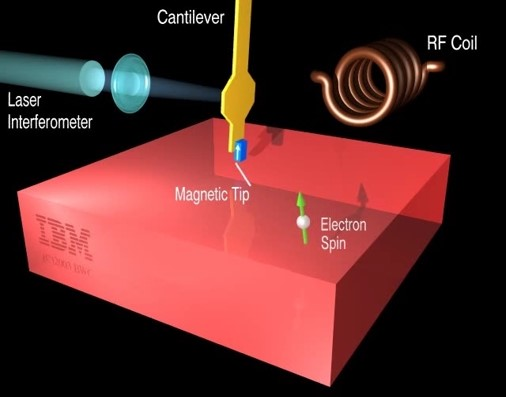
\includegraphics[height=90pt]{figures/AFM_RM.jpg}
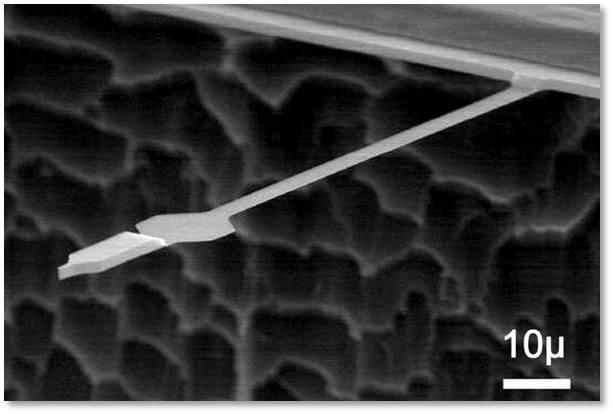
\includegraphics[height=90pt]{figures/AFM_quantilever.png}
\hfill
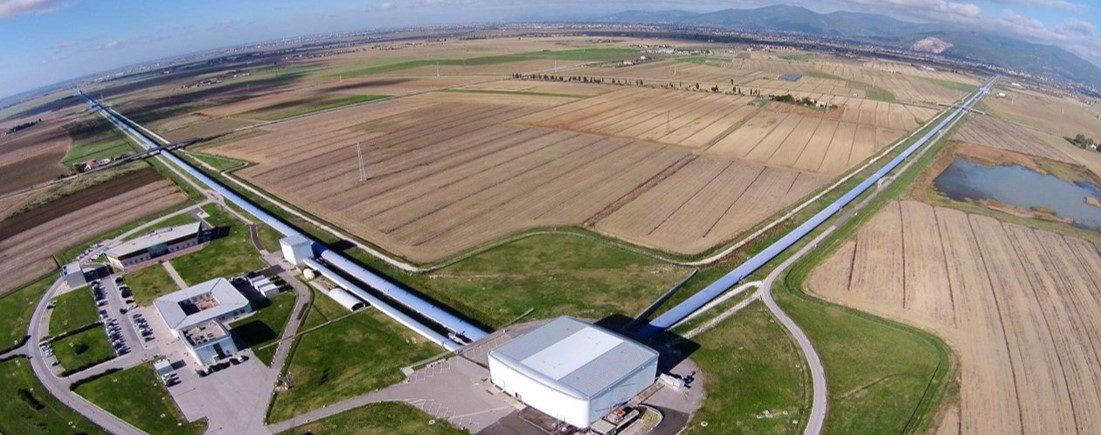
\includegraphics[height=90pt]{figures/virgo.jpg}
\caption{À gauche : résonance magnétique par mesure de force, capable de détecter des spins uniques, exerçant sur le micro-levier (au centre) une force de l'ordre de $\unit{10^{-18}}{\newton}$ (associé à un déplacement de $\unit{10^{-10}}{\meter}$).
À droite : interféromètre gravitationnel Virgo (Cascina, Italie), avec ses bras de \unit{3}{\kilo\meter}, capable de mesurer des déplacements relatifs de l'ordre de $10^{-21}$.}
\label{fig:displacement_measurement}
\end{figure}

\subsubsection{L'optomécanique : limite de sensibilité et contrôle de miroirs mobiles}

L'optomécanique est un domaine de recherche qui vient de la nécessité d'augmenter la sensibilité de ces détecteurs et qui s'intéresse au couplage entre la lumière et un miroir mobile.
Dans le cas des interféromètres gravitationnels, toute perturbation du détecteur se traduit comme un bruit qui, s'il n'est pas causé par le passage d'une onde gravitationnelle, dégrade la sensibilité de la mesure.
Par exemple, le bruit thermique au niveau des miroirs se traduit directement sous la forme d'un mouvement brownien qui conduit à utiliser des matériaux (silice) et des géométries permettant de concentrer les fluctuations de position autour des fréquences propres du système.
De cette façon, la sensibilité de l'appareil n'est dégradée qu'à certaines fréquences bien spécifiques, qu'il est possible de filtrer a posteriori.
La réduction de ces bruits classiques est maintenant telle que les bruits quantiques liés au laser lui même deviennent limitants.

D'une part, le \textbf{bruit quantique de phase} se traduit directement sur la mesure puisque ces fluctuations sont décorrélées entre les deux bras de l'interféromètre.
D'autre part, le \textbf{bruit quantique d'intensité} a deux conséquences sur la sensibilité de la mesure : un bruit direct sur l'intensité mesurée à la sortie du détecteur et des fluctuations de la force de \textbf{pression de radiation} qui s'exerce sur les miroirs de l'interféromètre et qui se traduit en bruit de position.
C'est l'action en retour de la mesure, prédite depuis les années 80, qui a contribué à lancer les recherches autour de l'optomécanique.
Dans un intérferomètre de Michelson, le déplacement $\delta x$ d'un miroir est donc associé à un déphasage
\begin{equation}
\delta \varphi = \delta \varphi ^\mathrm{phase} _\mathrm{q} + \frac{4\pi}{\lambda} ( \delta x + \delta x ^\mathrm{rad} _\mathrm{q} + \delta x_\mathrm{c}),
\end{equation}
où $\delta \varphi ^\mathrm{phase} _\mathrm{q}$ est le bruit quantique de phase, $\delta x ^\mathrm{rad} _\mathrm{q}$ le bruit de position associé au bruit d'intensité et $\delta x_\mathrm{c}$ regroupe les bruits classiques (thermique, sismique, électronique, etc.).
L'amplitude du bruit quantique de phase est inversement proportionnelle à l'amplitude du champ lumineux et peut donc être réduite en augmentant l'intensité du laser ce qui explique l'utilisation de puissances optiques importantes ($\sim \unit{100}{\kilo\watt}$ dans les cavités).
Au contraire, l'amplitude du bruit de pression de radiation est proportionnelle à l'amplitude du champ.
Elle est aussi modulée par la réponse mécanique du système, ce qui résulte en un compromis à l'origine de la limite quantique standard : à chaque fréquence correspond une puissance laser optimale qui égalise le bruit de pression de radiation et le bruit de phase.

Si l'effet de la pression de radiation peut s'avérer néfaste pour la sensibilité des mesures de grande précision, on peut également l'exploiter pour contrôler les degrés de liberté mécaniques d'un miroir mobile.
C'est ainsi qu'au cours des vingt dernières années, de nombreux systèmes optomécaniques ont été développés avec des applications très variées (capteurs de force, de masse, de température, transducteurs optique-microonde, ponderomotive squeezing, etc.).
Une des applications fondamentales de ces systèmes est l'observation d'effets quantiques sur des objets de plus en plus massifs, avec notamment l'observation en 2011 du premier refroidissement vers l'état quantique fondamental d'un oscillateur mécanique (de masse effective $m_\mathrm{eff} = \unit{50}{pg}$) couplé à une cavité microonde.
À travers l'utilisation d'oscillateurs mécaniques de masses effectives intermédiaires ($m_\mathrm{eff} \approx \unit{100}{\micro\gram}$, grande devant celle des systèmes utilisés pour le refroidissement mais petite devant celle des miroirs des interféromètres gravitationnels), l'objectif de ma thèse était donc double :
\begin{enumerate}
\item \textbf{Refroidir un oscillateur mécanique macroscopique dans son état quantique fondamental}, avec une masse trois ordres de grandeur plus importante que les précédentes expériences, et en particulier proche de la masse de Planck ($m_\mathrm{P}=\unit{22}{\micro\gram}$) au delà de laquelle les effets de décohérence liés à la gravité deviennent significatifs ;
\item Préparer un système modèle qui permette d'\textbf{étudier les limites de sensibilité de la mesure de petits déplacements liés au bruit de pression de radiation}, tout en restant beaucoup plus compact que les interféromètres gravitationnels et leur miroirs ($m_\mathrm{eff}\approx\unit{50}{\kilo\gram}$).
\end{enumerate}
Le premier point est un pré-requis du deuxième puisque le système étudié est limité par le bruit thermique : afin d'observer le bruit de pression de radiation, il est nécessaire de réduire le mouvement brownien de plus de six ordres de grandeurs, ce qui revient à refroidir l'oscillateur mécanique proche de son état quantique fondamental.

Le refroidissement de l'oscillateur mécanique se fait en utilisant les techniques de l'optomécanique en cavité.
Il est pour cela nécessaire de disposer de \textit{bons} oscillateurs mécaniques qui seront décrits dans un premier temps.
Pour mesurer précisément leurs déplacements, ces oscillateurs sont utilisés comme l'un des miroirs d'une cavité optique de grande finesse dont les contraintes et la mise en pratique sera présentée.
L'utilisation du couplage optomécanique dans une telle cavité est ensuite détaillé pour le refroidissement de l'oscillateur.
Le bon fonctionnement de l'expérience nécessite plusieurs boucles de contrôle qui sont réalisées notamment à l'aide de micro-contrôleurs interfacés en Python.
Les principaux résultats obtenus au cours de ma thèse sont finalement exposés avant une brève mise en perspective dans le cadre de l'amélioration de la sensibilité des détecteurs d'ondes gravitationnelles.

\subsection{L'oscillateur mécanique, caractérisation et thermométrie}

Bien que les géométries des oscillateurs mécaniques soient très variées, son comportement est très bien décrit par un système \{masse, ressort\} amorti (masse effective $m_\mathrm{eff}$, pulsation propre $\Omega_m$ et amortissement $\Gamma_m$) soumis à des forces extérieures de résultante $F_\mathrm{ext}$, si bien que l'équation du mouvement de l'oscillateur s'écrit
\begin{equation}
m_\mathrm{eff} \frac{d^2 x(t)}{\d t^2} + m_\mathrm{eff}\Gamma_m \frac{d x(t)}{\d t} + m_\mathrm{eff} \Omega_m^2 x(t) = F_\mathrm{ext}(t).
\end{equation}
Son comportement fréquentiel se déduit dans l'espace de Fourier de la susceptibilité mécanique $\chi[\Omega]$ de l'oscillateur, avec
\begin{equation}
\chi[\Omega] = \frac{1}{m_\mathrm{eff}[(\Omega_m^2-\Omega^2)-i\Gamma_m\Omega]}.
\end{equation}
Dans la théorie de Langevin, le terme de dissipation $\Gamma_m$ se traduit par un couplage de l'oscillateur à son environnement, assimilé à un bain thermique à la température $T_\mathrm{env}$.
Il en résulte une force $F_\mathrm{T}$, dont le spectre est lié à la partie imaginaire de la susceptibilité mécanique par le théorème de fluctuations-dissipations, à l'origine du mouvement brownien de l'oscillateur.
On peut ainsi montrer que le spectre de déplacement de l'oscillateur à l'équilibre thermodynamique avec un tel bain thermique a une allure lorentzienne centrée sur la fréquence propre mécanique, dont l'intégration (l'aire sous la courbe) est directement liée au rapport $T_\mathrm{env}/m_\mathrm{eff}$.
La connaissance de l'un permet donc de déterminer l'autre à travers la mesure du spectre du mouvement brownien de l'oscillateur.
Le spectre est aussi d'autant plus piqué autour de la fréquence propre $\Omega_m$ que la dissipation est faible, ce qui conduit à utiliser des oscillateurs avec des facteurs de qualité mécaniques $Q=\Omega_m/\Gamma_m$ très élevés (supérieurs au million).

Cette description classique ne permet cependant pas d'expliquer le comportement de l'oscillateur aux très basses températures.
Il est alors nécessaire d'utiliser un modèle quantique, où le hamiltonien du système est simplement celui d'une masse $m_\mathrm{eff}$ dans un puits de potentiel à une dimension de pulsation $\Omega_m$.
La résolution de l'équation de Schrödinger conduit à une quantification des niveaux d'énergie du système sous forme de demi-entiers de $\hbar\Omega_m$.
L'état du système peut alors être décrit en terme de niveau d'occupation exprimé en nombre de phonons
\begin{equation}
n_\mathrm{T} = \left[ e^\frac{T_Q}{T} -1\right]^{-1},
\label{eq:phonon_number}
\end{equation}
où la température quantique $T_Q$ est définie comme $T_Q = \hbar\Omega_m/k_B$.
En particulier, l'énergie minimale du système dans son état fondamental n'est pas nulle et conduit à un bruit de position appelé fluctuations de point zéro, dont l'amplitude $x_\mathrm{ZPF}$ est donnée par
\begin{equation}
x_\mathrm{ZPF}=\sqrt{\frac{\hbar}{2m_\mathrm{eff}\Omega_m}}.
\end{equation}
L'objectif de ma thèse peut alors être précisé puisqu'il s'agit de refroidir un oscillateur mécanique à une température inférieure à $T_Q$ pour laquelle le niveau d'occupation est inférieur à un phonon.

\begin{mep}
En première année de CPGE (PCSI ou MPSI), l'étude des propriétés classiques de ces oscillateurs pourrait me servir de fil rouge pour les cours de mécanique et en particulier pour l'étude de l'oscillateur harmonique amorti en régimes libre et forcé.
L'évolution de l'amortissement peut être reliée à la viscosité d'un fluide dans lequel est plongé l'oscillateur, celle de la fréquence reliée à la masse effective pour obtenir une balance, etc.
Ceci fourni nombre d'exemples pratiques d'utilisation de tels objets comme capteurs notamment.
La description fréquentielle de la réponse mécanique me semble également très pertinente pour donner aux étudiants une bonne intuition de ce qu'est un filtre passe-bas (par exemple) et pourrait ainsi être rapprochée de l'étude des filtres électroniques.

\noindent
Même si l'étude d'une particule dans un puits de potentiel harmonique n'est pas au programme de CPGE, l'étude quantique de ces systèmes pourrait faire l'objet d'une approche documentaire dans laquelle les étudiants seront amenés à effectuer la comparaison avec le cas d'un puits de potentiel de profondeur finie.
En MP, je pourrais aller jusqu'à l'étude statistique permettant de retrouver l'expression~\ref{eq:phonon_number} pour discuter de l'état du système en fonction de la température.
\end{mep}

\begin{figure}
\center
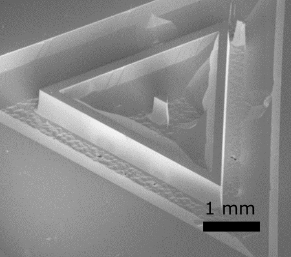
\includegraphics[height=90pt]{figures/micropillar.png}
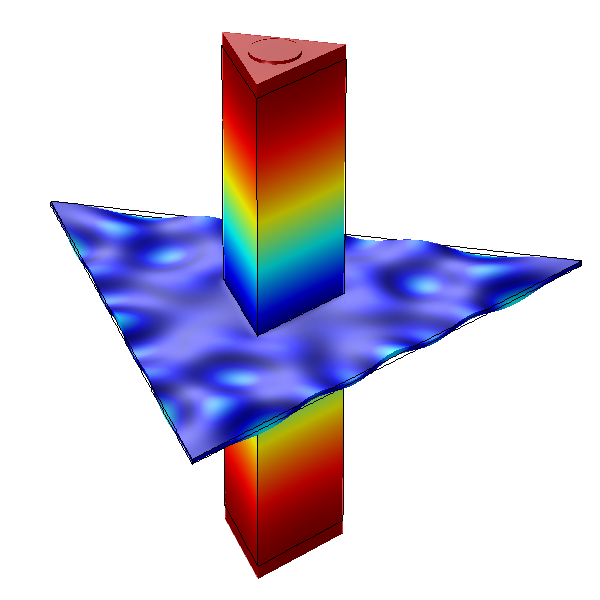
\includegraphics[height=90pt]{figures/micropillar_disp.png}
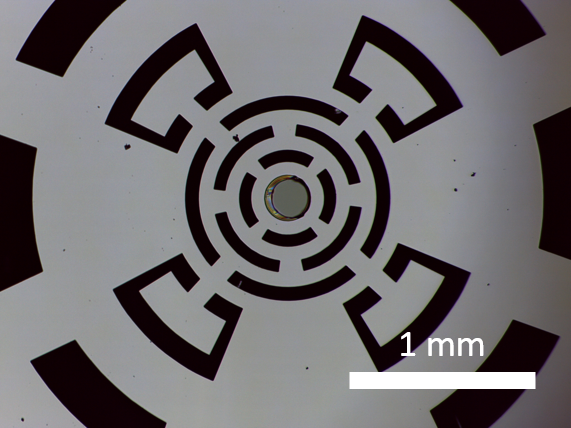
\includegraphics[height=90pt]{figures/microwheel.png}
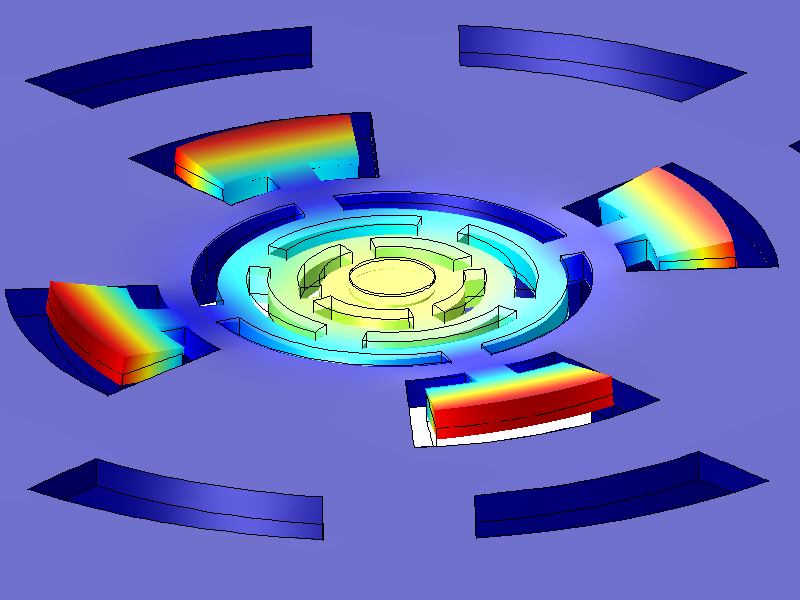
\includegraphics[height=90pt]{figures/microwheel_disp.png}
\caption{À gauche : image obtenue par microscopie électronique d'un micro-pillier en quartz et simulation du mode propre fondamental de compression utilisé.
À droite : image obtenue par microscopie optique d'un micro-disque en silicium et simulation du mode propre utilisé.
Les simulations sont réalisées avec COMSOL (simulation par éléments finis) et le code couleur correspond au déplacement de la structure (du bleu au rouge, où le rouge correspond au déplacement maximal).}
\label{fig:resonators}
\end{figure}

Au cours de ma thèse, j'ai utilisé deux types d'échantillons visibles sur la figure~\ref{fig:resonators} :
\begin{itemize}
\item \textbf{micro-pilier} : un oscillateur en quartz (micro-fabriqué en collaboration avec l'ONERA, Paris) sous la forme d'un pilier de section triangulaire (\unit{240}{\micro\meter} de côté, \unit{1}{\milli\meter} de long).
Il est suspendu en son milieu par une membrane d'environ \unit{10}{\micro\meter} d'épaisseur et un micro-miroir de très haute réflectivité est déposé sur l'une de ses extrémités (en collaboration avec le LMA, Lyon), $m_\mathrm{eff}=\unit{33{,}5}{\micro\gram}$, $\Omega_m=2\pi\times\unit{3{,}6}{\mega\hertz}$ et $Q=10^7$ : $T_{Q,\mathrm{pilier}} = \unit{200}{\micro\kelvin}$ ;
\item \textbf{micro-disque} : un disque en silicium (en collaboration avec l'UniFI, Italie) d'environ $\unit{200}{\micro\meter}$ de diamètre sur lequel est déposé un miroir de très haute réflectivité, $m_\mathrm{eff}=\unit{112}{\micro\gram}$, $\Omega_m=2\pi\times\unit{280}{\kilo\hertz}$ et $Q=10^6$ : $T_{Q,\mathrm{disque}} = \unit{10}{\micro\kelvin}$.
\end{itemize}
Avant d'être utilisés pour les expériences de refroidissement, les échantillons doivent être caractérisés soigneusement, notamment pour la thermométrie à basse température.
Leur réponse mécanique est tout d'abord calibrée à l'aide d'une excitation réalisée grâce à une cale piézoélectrique par exemple (observation des différents modes mécaniques, mesure de $\Omega_m$, $Q$).
Leur masse effective $m_\mathrm{eff}$ est ensuite obtenue en mesurant par interférométrie optique le mouvement brownien de l'oscillateur à température ambiante.
Les problèmes de thermalisation sont alors très faibles et la température de l'échantillon est donc très proche de celle obtenue grâce à un simple thermomètre situé à proximité.
Les paramètres $\Omega_m$ et $Q$ dépendent fortement du régime de température et de pression  : l'échantillon est donc placé dans un cryostat à circulation d'hélium permettant d'atteindre rapidement des températures de l'ordre du kelvin et des pressions inférieures à $\unit{10^{-5}}{\milli bar}$.
Des spectres obtenus lors de telles mesures sont visibles sur la figure~\ref{fig:thermal_noise}.

\begin{mep}
Les principes des techniques employées pour la caractérisation de nos échantillons peuvent sans difficulté être utilisés pour, par exemple, la caractérisation mécanique d'un diapason, ou d'un verre vibrant.
En terminale scientifique, je pourrai par exemple proposer une approche expérimentale afin de caractériser mécaniquement ces objets.
Il sera alors possible de discuter de l'évolution des grandeurs caractéristiques (fréquence et amortissement notamment) du système en fonction de paramètres comme la température, la masse effective, l'amortissement, etc.
Je pourrai ensuite montrer aux élèves comment ces techniques sont utilisées en recherche grâce à une visite du laboratoire.
\end{mep}

\begin{figure}
\center
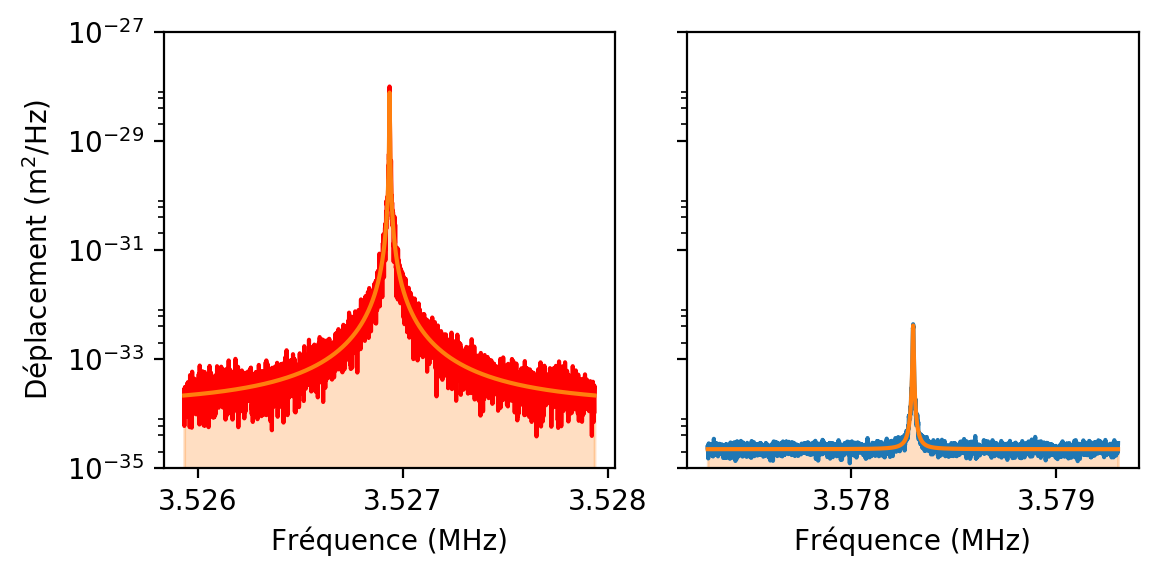
\includegraphics[scale=0.75]{figures/thermal_peak_def_filled.png}
\caption{Spectres du bruit de position d'un micro-pilier en cavité dû au mouvement brownien de l'oscillateur.
Le déplacement est exprimé en $\meter\squared\per\hertz$ car on s'intéresse ici non à l'amplitude mais plutôt à la puissance du bruit de position, normalisé par la bande passante de l'analyseur de spectre.
La figure de gauche est obtenue à température ambiante ($\sim\unit{300}{\kelvin}$) alors que celle de droite est obtenue en cryogénie à $\sim\unit{30}{\milli\kelvin}$.
Le refroidissement de l'échantillon s'accompagne d'un déplacement de sa fréquence de résonance d'une augmentation de son facteur de qualité (en raison de la dépendance en température des propriétés mécaniques des matériaux utilisés), ainsi que d'une diminution de l'aire sous le pic associée à la réduction du mouvement brownien, proportionnelle à la température.}
\label{fig:thermal_noise}
\end{figure}

\subsection{Une cavité optique pour augmenter la sensibilité}

Comme on l'a évoqué précédemment, la mesure des déplacements de l'oscillateur est réalisée par interférométrie optique : un faisceau laser se réfléchissant sur un miroir mobile acquiert un déphasage $\delta\varphi$ qui dépend du déplacement $\delta$ du miroir.
La sensibilité $\delta\varphi / \delta x$ de cette mesure dépend du protocole de détection employé.
Par exemple dans le cas d'un interféromètre de Michelson dont l'un des bras se termine par le miroir mobile, la sensibilité vaut $4\pi/\lambda$ et ne dépend que de la longueur d'onde du laser.
L'utilisation d'une cavité de grande finesse $\cal{F}$ permet d'amplifier le déphasage : si la cavité est résonante avec le laser, on a
\begin{equation}
\delta \varphi = 8\pi{\cal{F}}\frac{\delta x}{\lambda},
\end{equation}
car la lumière effectue alors en moyenne ${\cal{F}}$ allers-retours dans la cavité.
Le déphasage est ensuite traduit en variation d'intensité en faisant interférer ce faisceau signal avec un faisceau de référence, appelé oscillateur local.

Plusieurs détections ont ainsi été implémentées, possédant chacune leurs avantages et inconvénients en terme de sensibilité et simplicité de mise en œuvre.
Pour les caractérisations préliminaires des échantillons un simple Michelson est suffisant puisque on étudie alors un régime forcé (oscillations forcées grâce à une cale piézoélectrique) où l'amplitude des déplacement est grande.
En revanche, pour les mesures de mouvement brownien, la sensibilité du Michelson n'est plus suffisante et il est nécessaire d'utiliser une cavité Fabry-Perot, dont l'un des miroirs est l'oscillateur mécanique.
On peut alors détecter la lumière réfléchie par la cavité :
\begin{itemize}
\item détection directe : si la cavité est légèrement désaccordée par rapport au laser, une variation de sa longueur est directement responsable de variations de l'intensité intracavité.
Le déplacement de l'oscillateur est ainsi relié à l'intensité réfléchie par la cavité ;
\item détection homodyne : si la cavité est résonante avec le laser, aucune variation d'intensité n'est mesurable mais la sensibilité $\delta\varphi/\delta x$ est maximale.
En faisant interférer le faisceau réfléchi par la cavité avec un faisceau de référence dans un interféromètre de Michelson, on observe alors les variations de l'intensité transmise par l'interféromètre.
L'utilisation d'une détection balancée permet d'atténuer fortement le bruit classique, ce qui autorise des mesures limitées par les bruits quantiques. 
\end{itemize}
Le principe de ces détections est résumé sur la figure~\ref{fig:detection_scheme}.
D'autres méthodes (Pound-Drever-Hall, détection hétérodyne, détection synchrone) sont aussi nécessaires mais elles ne seront pas présentées ici.

\begin{figure}
\center
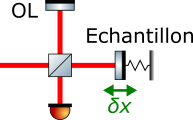
\includegraphics[scale=0.8]{figures/michelson_scheme.png} \hfill
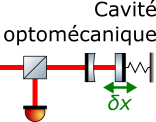
\includegraphics[scale=0.8]{figures/cavity_intensity_scheme.png}\hfill
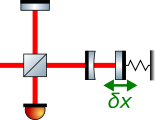
\includegraphics[scale=0.8]{figures/cavity_phase_scheme.png}
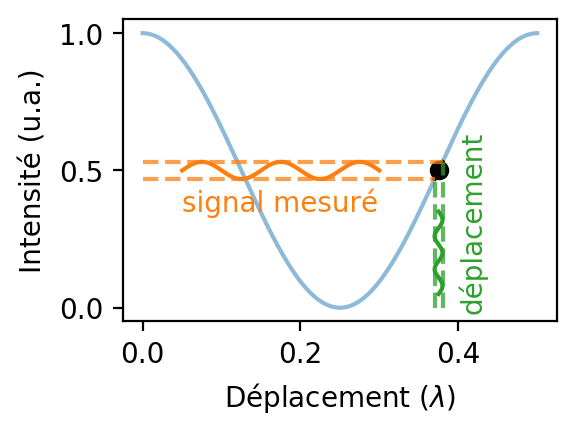
\includegraphics[scale=0.75]{figures/michelson_response.png}
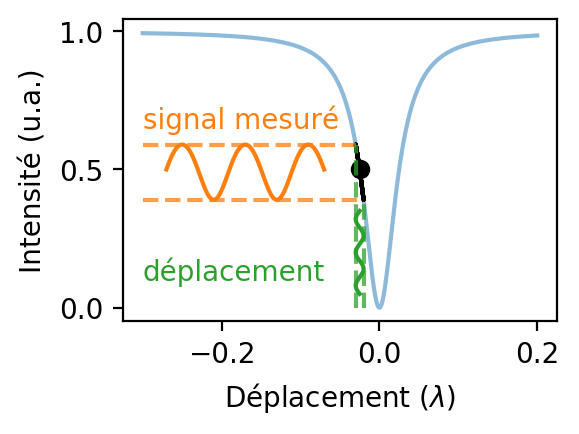
\includegraphics[scale=0.75]{figures/cavity_intensity_response.png}
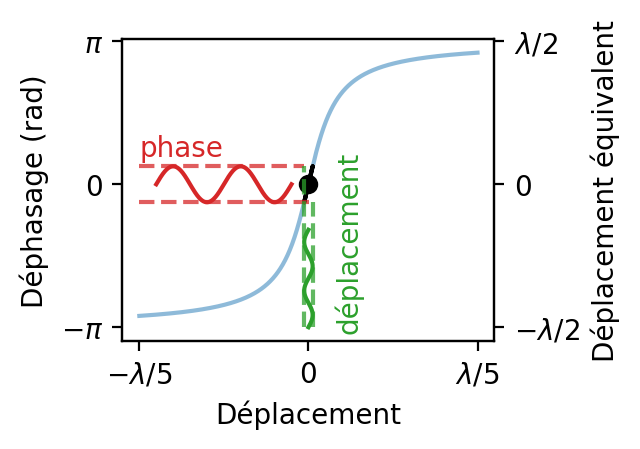
\includegraphics[scale=0.75]{figures/cavity_phase_response.png}
\caption{Schéma simplifié de trois dispositifs expérimentaux utilisés pour la mesure de petits déplacements.
De gauche à droite, mesure de l'intensité transmise par un interféromètre de Michelson, mesure de l'intensité réfléchie par une cavité Fabry-Perot (${\cal{F}}=20$) et mesure de la phase du faisceau réfléchi par la même cavité.}
\label{fig:detection_scheme}
\end{figure}

Compte tenu de la faible dimension des miroirs plans déposés sur les oscillateurs mécaniques, il est nécessaire d'utiliser comme miroir d'entrée de la cavité un miroir avec un rayon de courbure de l'ordre du millimètre (\uroc).
J'ai ainsi fabriqué par photoablation multiple à l'aide d'un laser $\mathrm{CO_2}$ des structures concaves, d'environ $\unit{200}{\micro\meter}$ de diamètre, avec des rayons de courbures et des ellipticités variés.
Un dépôt diélectrique de couches de silice $\mathrm{SiO_2}$ et d'oxyde de tantale $\mathrm{Ta_2O_5}$ réalisé au Laboratoire des Matériaux Avancés (Lyon) permet ensuite d'obtenir des miroirs ayant une transmission bien contrôlée entre 0 et $\unit{120}{ppm}$ typiquement.
J'ai ensuite développé un ensemble de pièces mécaniques en cuivre de haute pureté permettant un assemblage et un alignement rapide d'une cavité de $\unit{100}{\micro\meter}$ de longueur, constituée d'un échantillon (micro-pilier ou micro-disque) et d'un \uroc\ comme miroir d'entrée, qui permet un asservissement de la longueur de cavité sur le laser et compatible avec une utilisation dans un cryostat à dilution.
La cavité obtenue est visible sur la figure~\ref{fig:cavity}.

\begin{mep}
En deuxième année de CPGE, je pourrai me servir des nombreux dispositifs interférentiels utilisés (Michelson et Mach-Zender fibré ou non, Fabry-Perot) pour mettre en évidence l'importance de l'utilisation des interférences dans les mesures sensibles actuelles.
Certaines méthodes de détections utilisées impliquent une modulation/démodulation de l'information (le déplacement) sur une porteuse (le laser) qu'il est possible de rapprocher des méthodes employées dans les télécommunications avec une classe de PSI.
Je pourrai aussi proposer à des élèves de première un interféromètre imprimable en 3D piloté par Arduino, développé dans l'équipe, dans le cadre d'un projet expérimental et numérique de l'enseignement scientifique.
Ils mettraient ainsi en pratique des compétences variées : impression 3D, programmation, mesures et incertitudes.
\end{mep}

\begin{figure}
\center
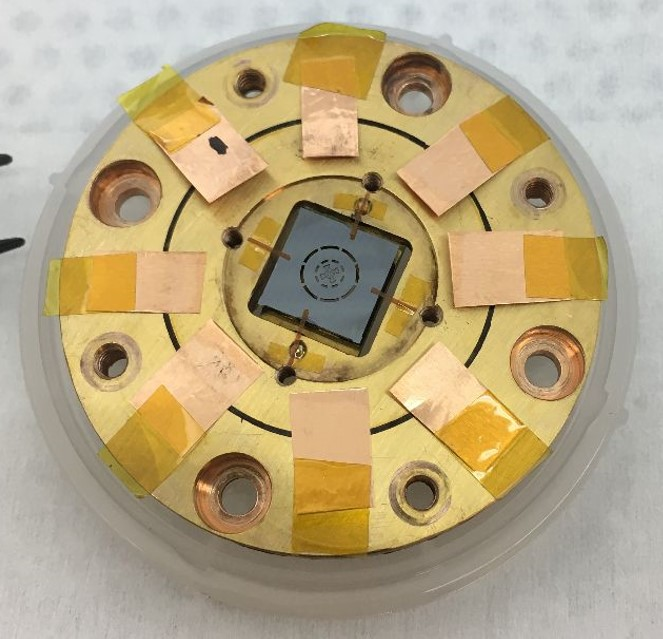
\includegraphics[height=130pt]{figures/cavity_microwheel.jpg}
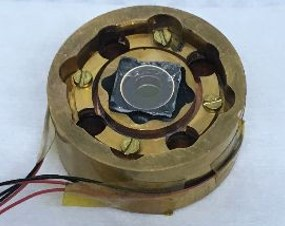
\includegraphics[height=130pt]{figures/cavity_uroc.jpg}
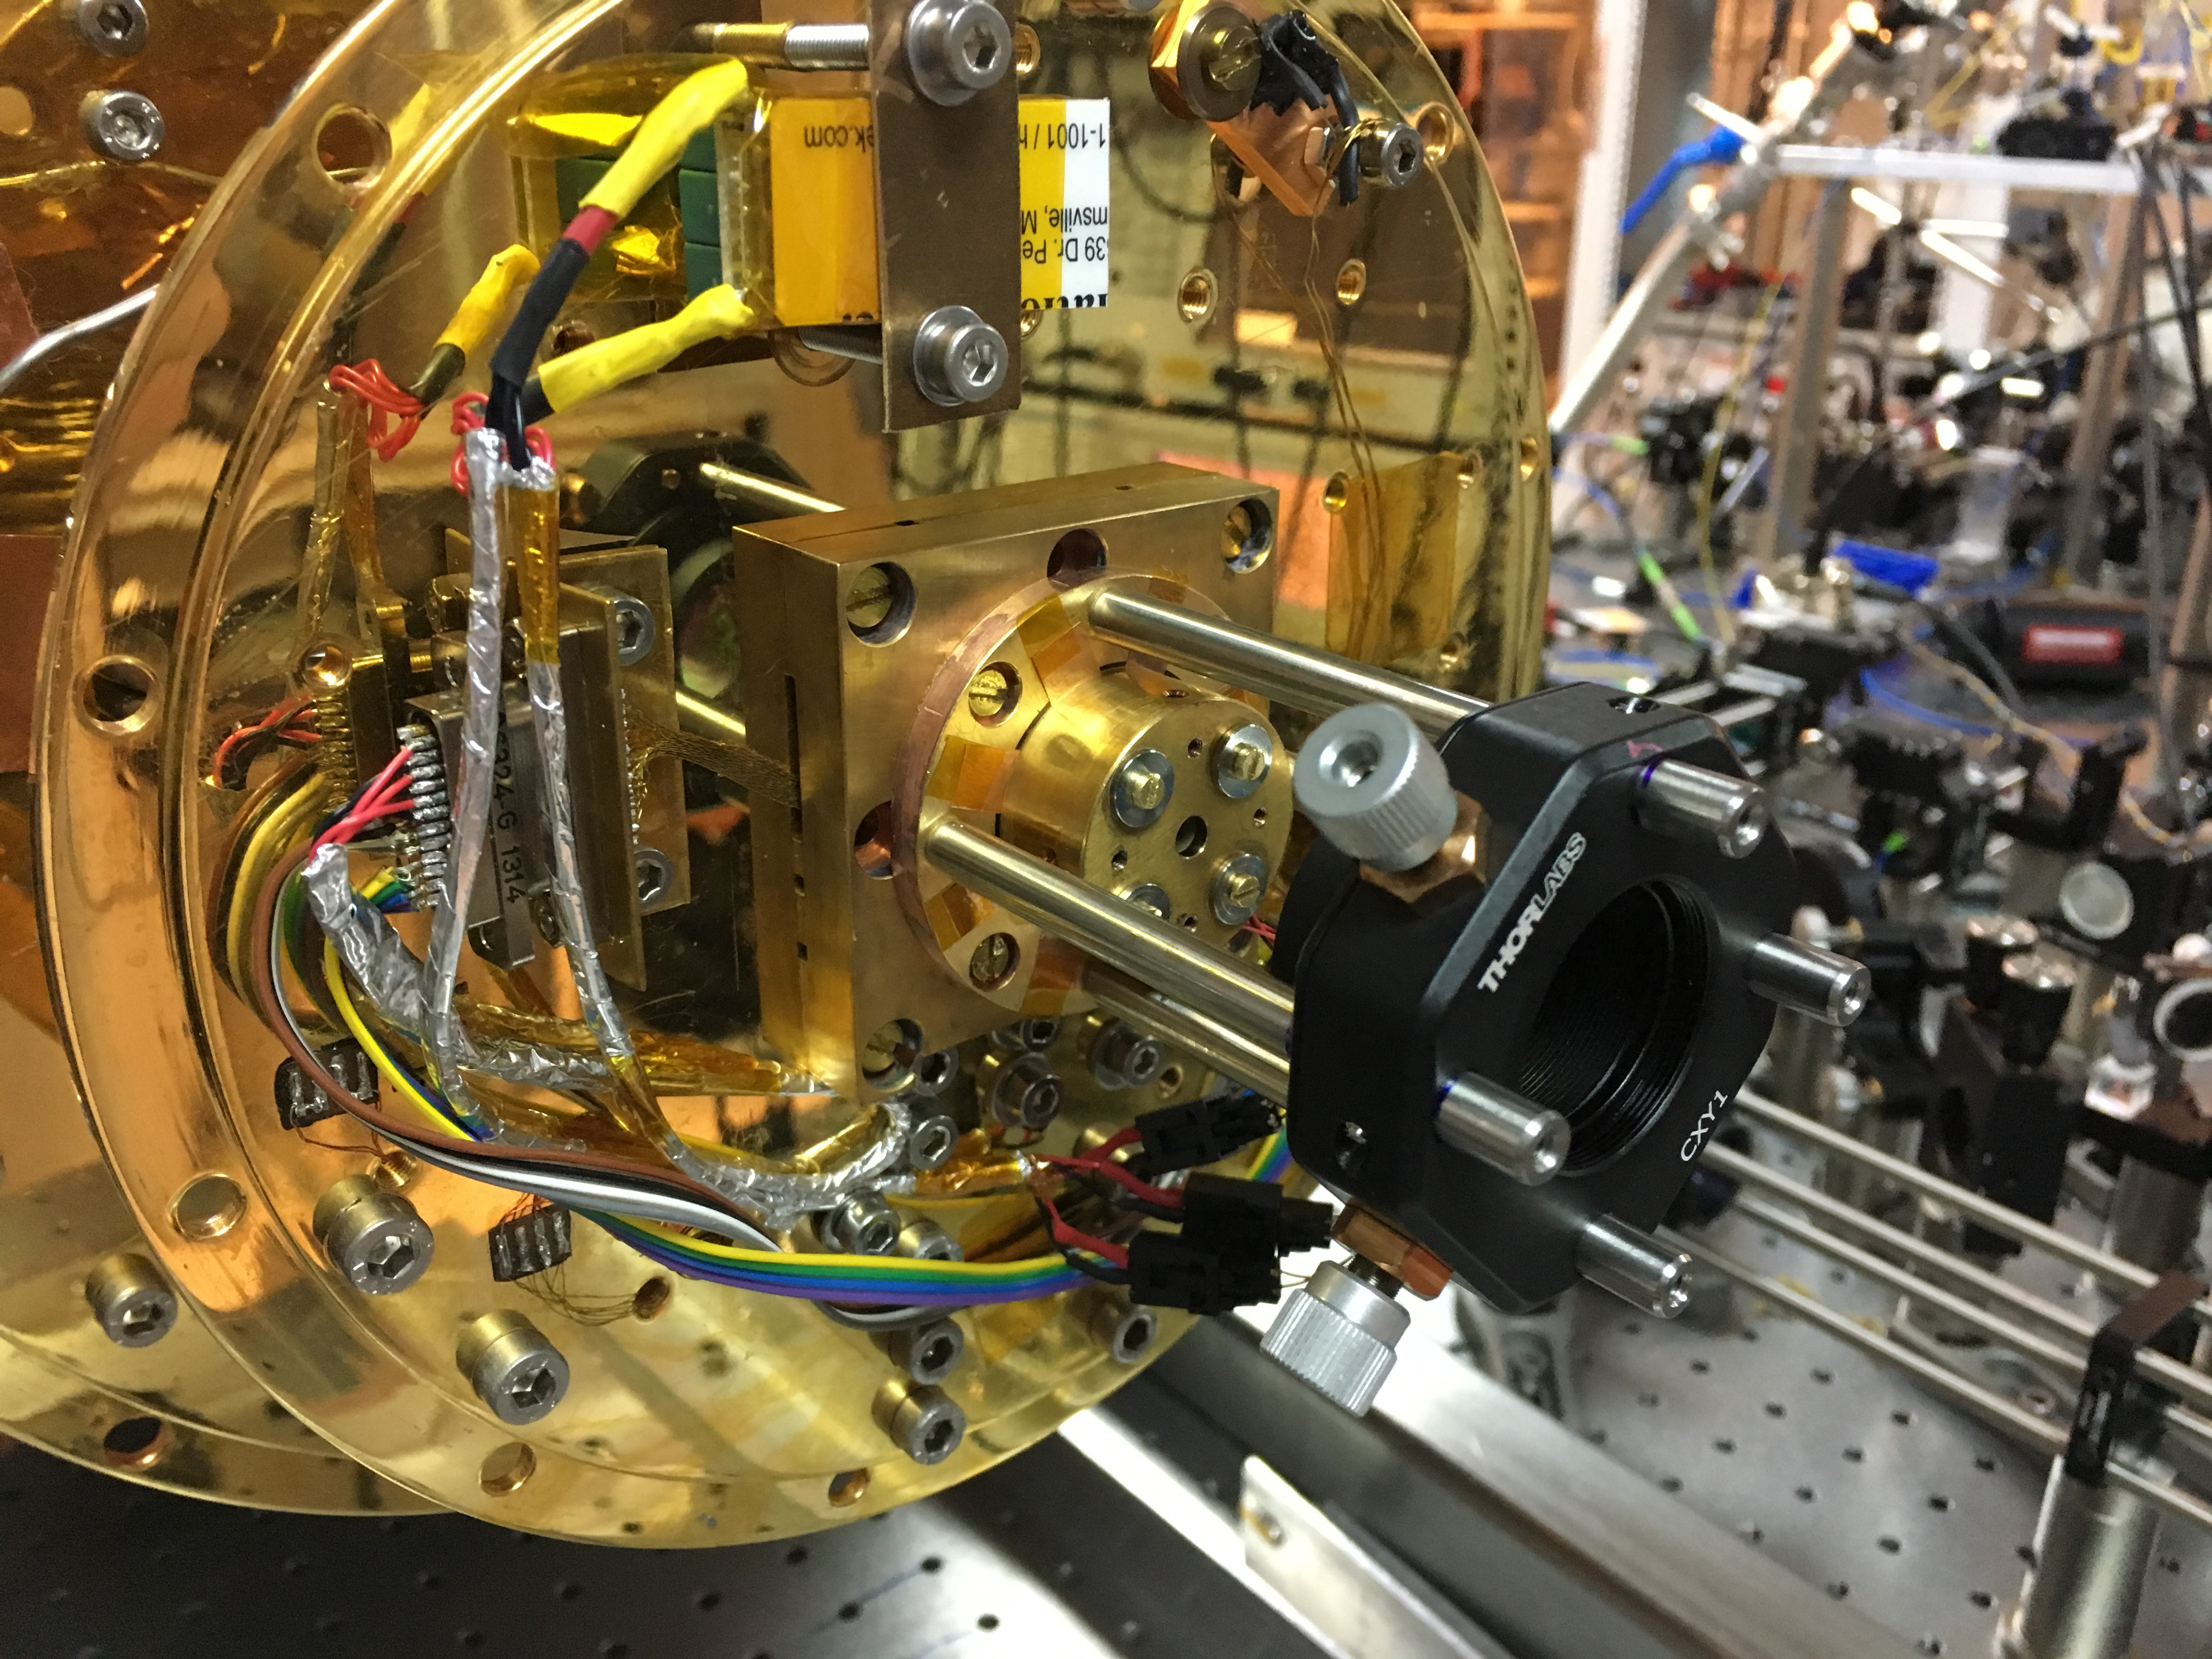
\includegraphics[height=130pt]{figures/IMG_1766.JPG}
\caption{La cavité est constituée de deux parties principales, avec l'oscillateur mécanique dans la première (à gauche : un micro-disque) et le miroir de couplage (\uroc) monté dans la seconde.
Les fils permettent de contrôler les cales piézoélectriques qui permettent l'asservissement en longueur de la cavité.
À droite, on peut voir la cavité assemblée et montée sur le dernier étage du cryostat à dilution.
La lentille de courte focale permet de coupler le faisceau incident au mode fondamental $\mathrm{TEM_{00}}$ de la micro-cavité.}
\label{fig:cavity}
\end{figure}

\subsection{Refroidissement par rétroaction par pression de radiation}

Pour préparer les oscillateurs mécaniques dans leur état quantique fondamental, il est nécessaire d'atteindre des températures inférieures au mK.
L'utilisation d'un cryostat à circulation d'hélium permet de refroidir les échantillons à une température de quelques kelvin suffisante pour une caractérisation préliminaire de leurs propriétés mécaniques, mais trop élevée pour espérer atteindre le régime quantique.
C'est donc à l'aide d'un cryostat à dilution fonctionnant avec un mélange $\mathrm{^4He/^3He}$ que la cavité de mesure est tout d'abord refroidie jusqu'à \unit{30}{\milli\kelvin}.

\begin{mep}
Le fonctionnement de ces machines thermiques peut être abordé en PC dans le cadre d'une approche thermodynamique simplifiée.
Les problématiques liées à la conception du cryostat dans les phases préliminaires de l'expérience (enceinte sous vide, utilisation de matériaux de conductivités thermiques adaptées, accès optiques limitant le chauffage par rayonnement du corps noir) peuvent servir à illustrer les différents transferts thermiques qu'il est nécessaire de maitriser pour obtenir ces températures cryogéniques.
\end{mep}

Pour refroidir d'avantage l'oscillateur mécanique, il est ensuite possible d'exploiter les techniques propres l'optomécanique en cavité.
On peut par exemple exploiter directement le couplage optomécanique dans une cavité légèrement désaccordée ($\omega_\mathrm{L}<\omega_\mathrm{cav}$) :
\begin{itemize}
\item si un déplacement du miroir mobile conduit à un allongement de la cavité, sa fréquence de résonance $\omega_\mathrm{cav}$ diminue ce qui augmente le désaccord et diminue l'intensité intracavité : la pression de radiation est alors moins forte sur le miroir mobile ce qui a tendance à le ramener vers sa position d'équilibre ;
\item au contraire, si ce déplacement conduit à une cavité plus courte, $\omega_\mathrm{cav}$ augmente ce qui diminue le désaccord et augmente l'intensité intracavité : la pression de radiation est alors plus grande ce qui repousse le miroir vers sa position d'équilibre.
\end{itemize}
Cet auto-refroidissement a été exploité et a conduit un refroidissement jusqu'à un taux d'occupation de 20 phonons, limité par la puissance injectable dans la cavité.

\begin{figure}
\center
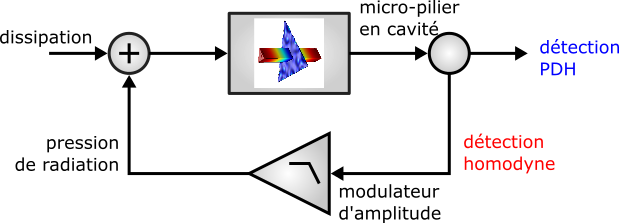
\includegraphics[scale=0.5]{figures/feedback_cooling.png}
\caption{Schéma de principe du refroidissement par rétroaction.
Le couplage à un bain thermique $T_\mathrm{env}$ en raison de la dissipation mécanique $\Gamma_m$ de l'oscillateur se traduit par un mouvement brownien du micro-pilier, qui peut être détecté optiquement en exploitant la réponse de la cavité résonante.
Le signal obtenu est amplifié, filtré, et alimente un modulateur d'amplitude qui agit sur le pilier par l'intermédiaire de la pression de radiation.
Une mesure indépendante de la boucle de rétroaction est obtenue grâce à un deuxième faisceau, indépendant du précédent.}
\label{fig:feedback_scheme}
\end{figure}

Une autre méthode permet d'obtenir, à puissance optique égale, des taux de refroidissement plus important : le refroidissement par rétroaction.
C'est une méthode active qui consiste à appliquer sur le miroir mobile une force qui va compenser la force thermique décrite précédemment.
Un schéma de principe de cette méthode est représenté sur la figure~\ref{fig:feedback_scheme}.
En pratique, il est nécessaire de mesurer les déplacements de l'oscillateur pour appliquer une force proportionnelle à sa vitesse, analogue à un terme de frottement visqueux.

La rétroaction peut être appliquée grâce à de nombreux actuateurs (mécanique avec les cales piézoélectriques, électrostatique avec une antenne, etc.)
Dans notre expérience, on utilise la pression de radiation en modulant l'intensité du faisceau permettant la mesure de position de l'oscillateur.
Le modulateur d'amplitude présente en effet une fonction de transfert très plate dans une large gamme de fréquence et évite d'ajouter des connexions électriques à la cavité de mesure ce qui serait source de bruit et de chauffage.
Il est alors possible d'augmenter le refroidissement en augmentant le gain de la boucle de rétroaction, soit en travaillant avec une puissance optique plus importante, soit en augmentant la profondeur de la modulation d'amplitude.

Dans le cas d'une mesure parfaite, c'est-à-dire sans bruit donc avec une sensibilité infinie, une augmentation du gain $g$ se traduit toujours par un refroidissement du mode mécanique car seul le signal correspondant à ses déplacements est mesuré puis réinjecté dans la boucle.
En réalité, la sensibilité de la mesure est limitée (fluctuations de position du miroir d'entrée, bruit électronique et ultimement, bruit quantique de phase) et il existe un gain optimal $g_\mathrm{opt}$ pour lequel le mouvement brownien de l'oscillateur est équivalent au bruit de la mesure.
Pour $g>g_\mathrm{opt}$, on réinjecte le bruit de la mesure dans la boucle qui est transcrit en bruit de position sur l'oscillateur.
On observe alors dans le spectre du signal mesuré une diminution du bruit autour de la fréquence de résonance de l'oscillateur en dessous du bruit de mesure (squashing) car le bruit de mesure et les déplacements de l'oscillateur sont alors corrélés.
Même s'il est possible de tenir compte de cet effet pour extraire la température effective du mode mécanique, on souhaite avoir une mesure indépendante de la boucle de rétroaction qui donne directement accès à la température de l'oscillateur.
On injecte pour cela un deuxième faisceau dans la cavité, avec une polarisation orthogonale au premier qui permet d'obtenir une mesure directe des déplacements de l'oscillateur.
L'effet de squashing ne perturbe pas cette mesure car le bruit des deux détections est décorrélé.

\subsection{Contrôle de l'expérience : Arduino, RedPitaya et Python}

Le fonctionnement de l'expérience repose sur de nombreux asservissements :
\begin{itemize}
\item noise-eater pour la réduction du bruit classique d'intensité du laser ;
\item cavité de filtrage asservie en longueur sur le laser et stabilisée en température ;
\item asservissement de la longueur de l'oscillateur local des Michelson pour obtenir la sensibilité maximale à mi-frange ;
\item intensité des faisceaux utilisés pour les mesures ;
\item température des cryostats ;
\item cavité de mesure asservie en longueur sur le laser ;
\item boucle de rétroaction pour le refroidissement.
\end{itemize}
La plupart de ces asservissements sont réalisés numériquement (sauf le dernier, analogique) avec des micro-contrôleurs RedPitaya et la bibliothèque PyRPL (Python RedPitaya Lockbox), développée au sein de l'équipe.
Il est ainsi possible de piloter une grande partie de l'expérience depuis un PC, ce qui autorise grâce à un répertoire de scripts Python l'automatisation des séquences de mesures.
Le bon fonctionnement de ces asservissements repose en partie sur l'utilisation de nombreux filtres et d'amplificateurs analogiques et numériques (depuis la réalisation de photodiodes à haute efficacité quantique et faible bruit jusqu'à l'utilisation de simples filtres passe-bas)

Un expérience préliminaire à la réalisation des micro-cavités de mesure nécessitait de réaliser une cavité de longueur variable sur l'ensemble de sa zone de stabilité afin d'étudier les mécanismes de pertes optiques dans une cavité de grande finesse.
On a donc choisit de monter un des deux miroirs sur une translation micrométrique motorisée par un moteur pas à pas.
En vue d'automatiser les mesures, j'ai développé un contrôleur basé sur une carte Arduino (programme Arduino, interface Python et électronique) permettant le positionnement de la translation.

\begin{mep}
L'utilisation, l'amélioration et le développement de ces systèmes bouclés m'a permis de développer une compréhension par l'expérience de ces systèmes asservis, renforcée par la suite par une approche plus théorique.
Ceci me sera très utile pour aborder les systèmes bouclés avec des étudiants en PSI.
Les compétences que j'ai développées en programmation, électronique analogique et numérique ainsi qu'à travers l'utilisation de micro-contrôleurs me seront utiles pour illustrer mes cours de simulations, mais aussi pour guider par des élèves dans le cadre de l'enseignement scientifique.
L'utilisation de PyRPL et RedPitaya offre par ailleurs de nombreuses possibilités : grâce à une carte RedPitaya ($\sim\unit{200}{\text{\euro}}$) et du programme PyRPL (open source), on peut disposer d'un oscilloscope, d'un GBF, d'un analyseur de spectre, d'un analyseur de réseau et d'une boite d'asservissement (pour ne citer que les fonctionnalités déjà existantes).
Cette ressource pourrait être introduite comme évolution de l'Arduino à des élèves de lycée et exploitée dans le cadre de travaux pratiques en CPGE.
\end{mep}

\subsection{Principaux résultats obtenus}

Après avoir caractérisé les échantillons (micro-piliers et micro-disques), réalisé les micro-miroirs de couplage, développé un assemblage mécanique permettant d'obtenir une micro-cavité asservie et à basse température, amélioré la sensibilité des différentes détections et réduit les parasites les plus gênants, optimisé les différents asservissements, la cavité optomécanique est placée dans le cryostat à dilution puis refroidie vers \unit{30}{\milli\kelvin}.
Les deux faisceaux (de la boucle de rétroaction et indépendant) sont injectés simultanément dans la cavité et elle est asservie en longueur sur le laser.
On acquiert le spectre du bruit de position de l'oscillateur obtenu grâce aux deux détections, simultanément et en faisant varier le gain de la boucle de rétroaction au moyen d'atténuateurs analogiques.
Les résultats obtenus lors d'une telle mesure avec un micro-pilier sont visibles sur la figure~\ref{fig:feedback_cooling_pillar}.

Il a ainsi été possible de refroidir le \textbf{micro-pilier} jusqu'à une température de $\unit{1,0\pm 0,1}{\milli\kelvin}$, ce qui correspond à un taux d'occupation de $\mathbf{5,3 \pm 0,5}$ \textbf{phonons}.
Des limitations importantes principalement attribuées à la dégradation progressive de l'échantillon, conduisant à une mauvaise thermalisation et à des instabilités photothermiques nous ont conduit à utiliser un nouveau type d'oscillateur : les \textbf{micro-disques}.
Avec ces échantillons et en seulement quelques mois, il a été possible d'atteindre une température de \unit{0,7\pm 0,1}{\milli\kelvin} correspondant à un niveau d'occupation de $\mathbf{55\pm5}$ \textbf{phonons}, cette fois limité par le bruit de position du miroir d'entrée de la cavité.
À température comparable, le niveau d'occupation du micro-disque est dix fois plus élevé que celui le micro-pilier car la fréquence du mode propre des micro-disques est dix fois plus faible ($T_Q = \hbar\Omega_m/k_B$). 

\begin{figure}
\center
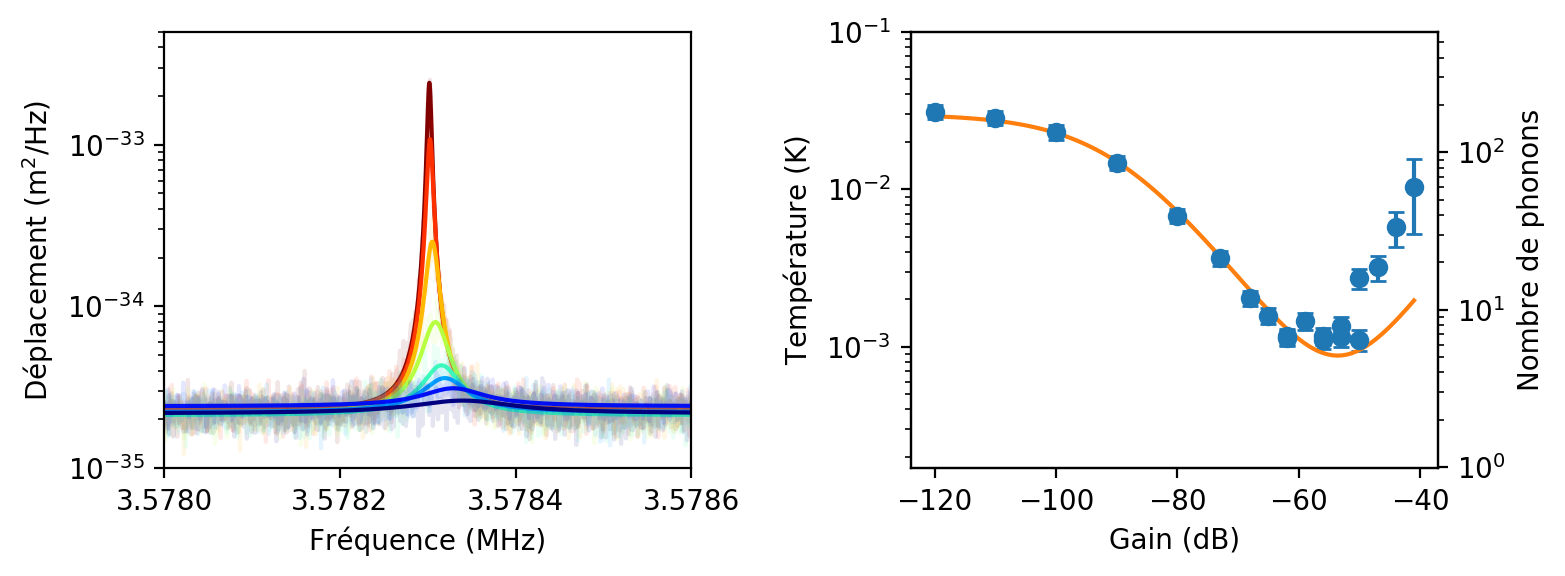
\includegraphics[scale=0.75]{figures/feedback_cooling_6phonons.png}
\caption{Refroidissement d'un micro-pilier proche de son état quantique fondamental.
À gauche : spectres du bruit de position obtenus avec la détection indépendante de la boucle de rétroaction obtenus pour différents gains (du rouge pour les gains faibles au violet pour $g_\mathrm{opt}$).
Les données expérimentales sont tracées en transparence et l'ajustement par le modèle théorique correspond aux courbes pleines.
À droite : températures effectives déduites des spectres obtenus avec la détection indépendante de la boucle de rétroaction.
La courbe orange correspond au modèle qui tient compte des paramètres de l'expérience.}
\label{fig:feedback_cooling_pillar}
\end{figure}

\subsection{Vers des mesures sous la limite quantique standard}

Les mesures présentées précédemment montrent deux limites de la sensibilité des mesures de petits déplacements : le bruit thermique (proche de la fréquence propre) et le bruit quantique de phase (partout ailleurs).
Compte tenu des puissances optiques utilisées et du niveau d'occupation thermique atteint, le bruit quantique de pression de radiation ne représente qu'une fraction du bruit de position mesuré (de l'ordre de \unit{1}{\%}).
Grâce aux développements réalisés sur la cavité optomécanique, une observation du bruit de pression de radiation (proportionnel à l'intensité lumineuse) devrait être possible, notamment en utilisant une puissance optique plus importante.
Il sera alors possible de démontrer une amélioration de la sensibilité de la mesure autour de la fréquence de résonance de l'oscillateur en remplaçant la source laser actuelle par une source de lumière comprimée.

Cette source est actuellement développée au sein de l'équipe et a déjà permis d'observer une réduction du bruit de phase de l'ordre de \unit{10}{dB}.
Il est aussi possible d'exploiter la réponse en phase d'une cavité optique (dite cavité de rotation) pour obtenir une réduction du bruit d'intensité à la fréquence de résonance de l'oscillateur (là où la réponse mécanique du système est maximale, et donc là où le bruit de pression de radiation est maximal) et une réduction du bruit de phase loin de la résonance (là où les fluctuations d'intensité ne perturbent pas la mesure).
Cette technique sera ensuite implémentée sur Virgo lors des prochaines campagnes de mesure afin d'étendre la portée du détecteur et ainsi observer plus d'évènements (augmenter la sensibilité de l'appareil par un facteur deux double sa porté, ce qui multiplie par huit le volume observable et donc la probabilité d'observer des sources d'ondes gravitationnelles).

\section{Enseignement, diffusion et vulgarisation}

\subsection{Enseignements}

Au cours de ma thèse, j'ai pu effectuer une mission d'enseignement qui m'a donné l'occasion de mettre en pratique plusieurs approches de l'enseignement.
Certaines étaient très classiques (comme les TP d'électromagnétisme) mais celle qui m'a le plus apporté est certainement celle de l'unité d'enseignement de physique expérimentale.
Cette UE ne contient aucun cours magistral et se compose d'une série de TP abordant l'électronique numérique et analogique ainsi que la programmation (Labview).
Chaque séance de TP est précédée d'un TD dont l'objectif est surtout de présenter aux étudiants le matériel qu'ils devront utiliser et d'aborder par l'expérience les concepts nouveaux.
Les TP les confrontent ensuite à des problématiques concrètes (réalisation d'un bras capable de détecter et saisir un objet par exemple) où ils doivent exploiter et se familiariser avec ces nouveaux concepts.
En fin de semestre, une compétition de robot est également organisée, dont les règles varient (combats de \og sumos\fg{}, positionner un drapeau au plus près d'une cible, etc.) et pour laquelle ils disposent d'une grande liberté.

Le parcours des étudiants que j'ai pu encadrer est souvent très disparate et il m'a parfois été difficile de m'adapter à chacun.
Leur investissement était toutefois réel et les séances très interactives.
Cette approche par l'expérience me semble essentielle puisqu'elle amène les étudiants à se poser eux-même les questions qui les font apprendre des notions nouvelles.
C'est une méthode d'enseignement très vivante dont je ne manquerai pas de m'inspirer en tant qu'enseignant.

\subsection{Vulgarisation : résonance et ondes gravitationnelles}

Le sujet et le contexte de ma thèse m'ont amené à plusieurs reprises à des activités de médiation auprès de publics très variés.
L'actualité récente depuis fin 2015 autour des ondes gravitationnelles a permis de mettre en avant tous les travaux liés à leur détections et à l'implication de telles observations.
J'ai ainsi été amené à réaliser des présentations sur l'histoire de la détection des ondes gravitationnelles devant des lycéens à l'occasion des Olympiades de physique, des fêtes de la Science organisées à Jussieu (Sorbonne Université), devant le personnel technique et administratif du LKB et finalement au Palais de la Découverte pour l'exposition \textit{Un chercheur, Une manip}.
La préparation, la présentation et les échanges qui ont suivi ces présentations ont été autant d'occasion de s'approprier différents aspects liés aux ondes gravitationnelles.
Ce sujet, par la variété des domaines qu'il fait intervenir, peut servir de fil conducteur et permette de rattacher les sujets abordés en cours à une actualité scientifique  qui promet de nombreux rebondissements.
On peut, sans exhaustivité, aborder les systèmes à deux points, l'oscillateur harmonique, l'interférométrie, les asservissements, le traitement du signal, etc.
La communauté LIGO/Virgo est très dynamique et offre des ressources qu'il est possible de réinvestir à tous les niveaux (articles, données, etc.).

A l'occasion du sujet \textit{Peut on casser un verre avec la voix ?} de l'émission E=M6, j'ai aussi mis en place une expérience permettant de casser un verre en le faisant vibrer à l'aide d'une source sonore.
Après avoir réalisé des simulations par éléments finis (COMSOL) comme on peut le voir sur la figure~\ref{fig:wine_glass}, on peut observer expérimentalement les différents modes propres d'un verre et visualiser les vibrations à l'aide d'un stroboscope.
Cette expérience permet notamment d'aborder l'analyse spectrale et le phénomène de résonance, qui pourrait faire l'objet d'une manipulation de TP (un peu bruyante certes) sans bien sûr aller nécessairement jusqu'à la rupture.

\begin{figure}
\center
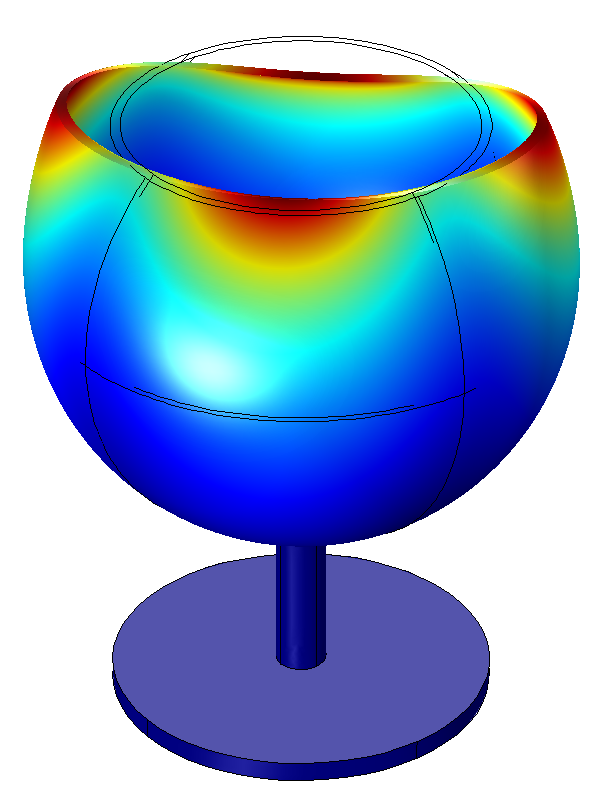
\includegraphics[height=100pt]{figures/wine_glass_f0.png}
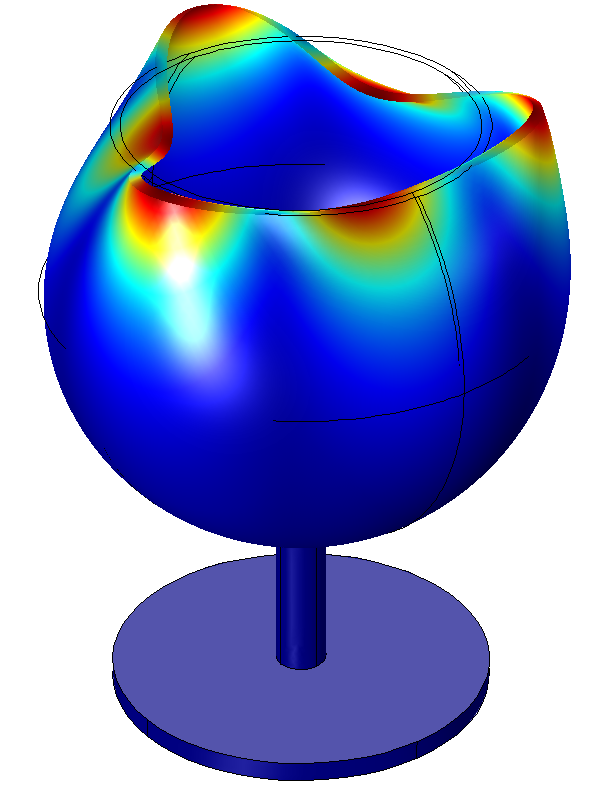
\includegraphics[height=100pt]{figures/wine_glass_f1.png}
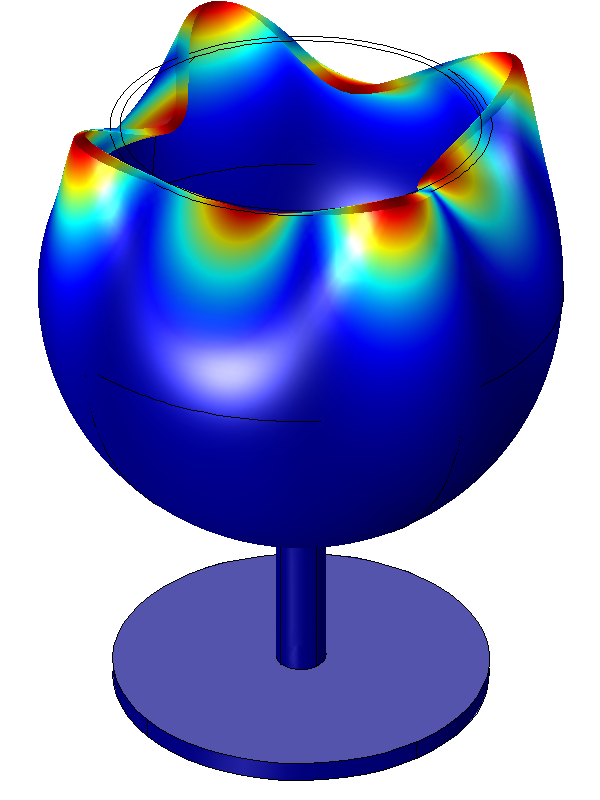
\includegraphics[height=100pt]{figures/wine_glass_f2.png}
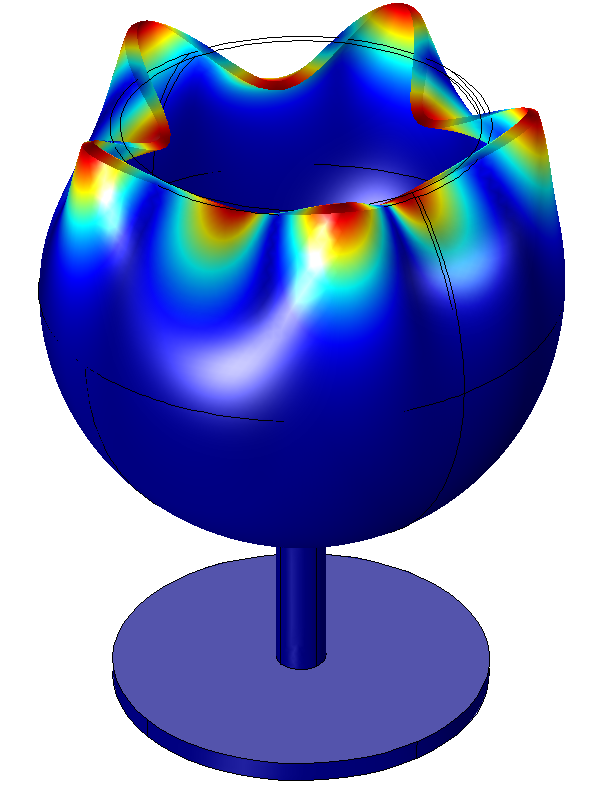
\includegraphics[height=100pt]{figures/wine_glass_f3.png}
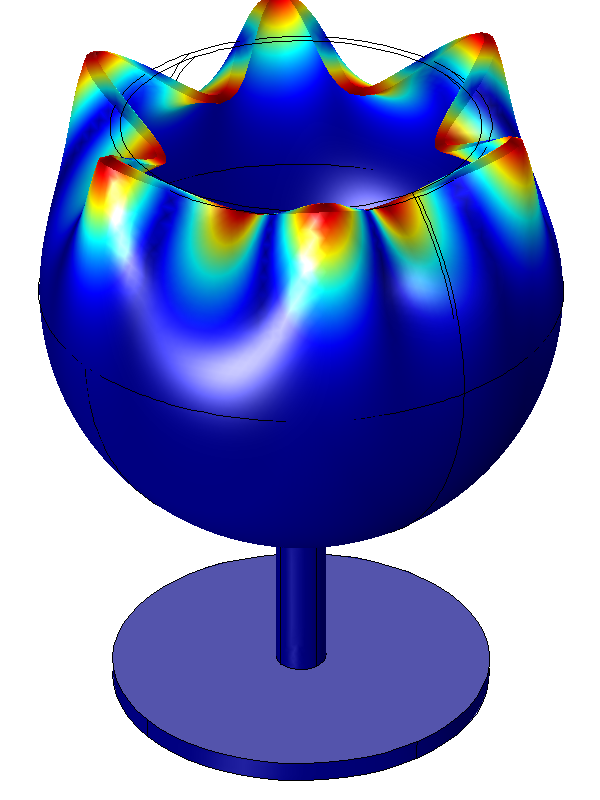
\includegraphics[height=100pt]{figures/wine_glass_f4.png}
\caption{Simulations des premiers modes de vibration d'un verre.}
\label{fig:wine_glass}
\end{figure}

\subsection{Aïkido}

En plus de mes activités scientifiques, j'ai aussi pratiqué l'Aikido que j'ai enseigné pendant quatre ans, notamment dans la section enfant/adolescent du dojo Shinkai.
Pour cela, j'ai passé le brevet fédéral (diplôme d'enseignement de la FFAB) ce qui m'a donné l'opportunité de développer une autre approche de la transmission de savoirs.
Une des principales difficultés rencontrées est là encore la diversité des pratiquants (âge, morphologie et ancienneté) à laquelle il est nécessaire de s'adapter afin d'obtenir une bonne cohésion du groupe et d'amener les éléments nécessaires à la progression de chacun.
Cette problématique est aussi à mon sens une richesse de l'enseignement.
En plus de l'équilibre qu'ils m'apportent, la pratique et l'enseignement de l'Aïkido seront des atouts importants en tant qu'enseignant.

%\bibliographystyle{custom-bib/thesis}
\bibliographystyle{abbrv}
\nocite{*}
\bibliography{biblio}

\end{document}